\documentclass[landscape]{standalone}

\usepackage{tikz}
\usepackage{pgf-umlcd}

\begin{document}

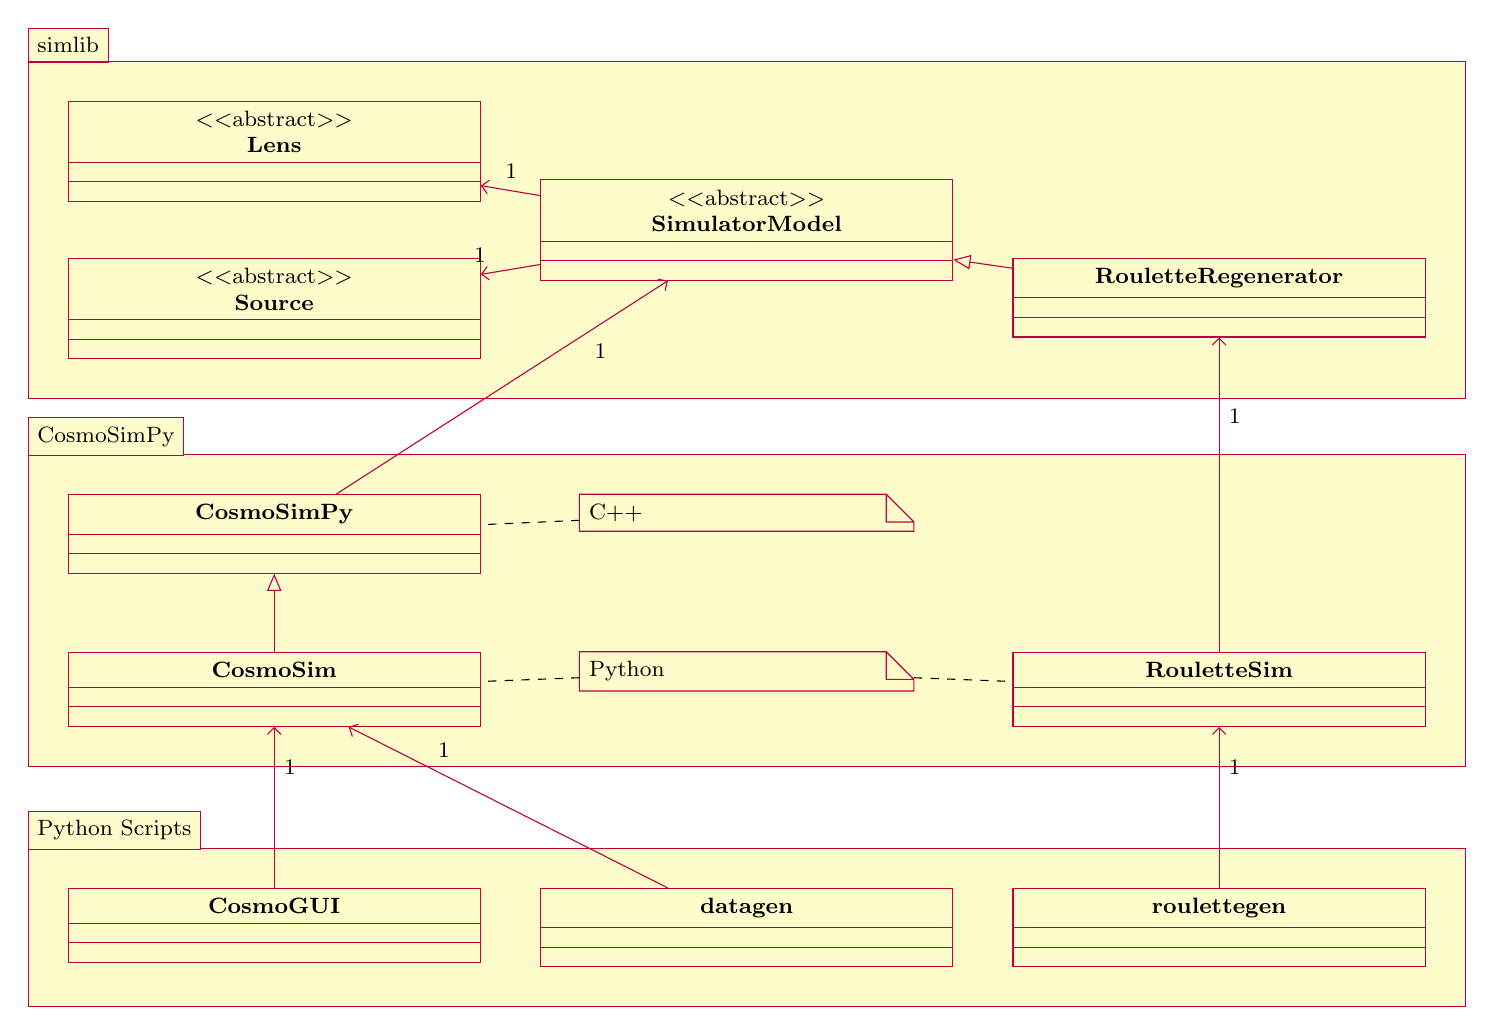
\begin{tikzpicture}
       \tikzstyle{every node}=[font=\footnotesize]

   \begin{package}{simlib}

      \begin{abstractclass}{SimulatorModel}{0 , 11}
      \end{abstractclass}

      \begin{abstractclass}{Lens}{-6 , 12}
      \end{abstractclass}
      \unidirectionalAssociation{SimulatorModel}{}{1}{Lens}

      \begin{abstractclass}{Source}{-6 , 10}
      \end{abstractclass}
      \begin{class}{RouletteRegenerator}{6 , 10}
	 \inherit{SimulatorModel}
      \end{class}
      \unidirectionalAssociation{SimulatorModel}{}{1}{Source}

   \end{package}

   \begin{package}{CosmoSimPy}
      \begin{class}{CosmoSimPy}{-6 , 7}
      \end{class}
      \umlnote (note1) at (0,7) { C++ };
      \unidirectionalAssociation{CosmoSimPy}{}{1}{SimulatorModel}
      \begin{class}{CosmoSim}{-6 , 5}
         \inherit{CosmoSimPy}
      \end{class}
      \umlnote (note2) at (0,5) { Python };
      \draw [dashed] (note1) -> (CosmoSimPy) ;
      \draw [dashed] (note2) -> (CosmoSim) ;
      % \begin{class}{RouletteSimC++}{6 , 7}
      % \end{class}
      % \draw [dashed] (note1) -> (RouletteSimC++) ;
      \begin{class}{RouletteSim}{6 , 5}
         % \inherit{RouletteSimC++}
      \end{class}
      \draw [dashed] (note2) -> (RouletteSim) ;
      \unidirectionalAssociation{RouletteSim}{}{1}{RouletteRegenerator}
   \end{package}

   \begin{package}{Python Scripts}
   \begin{class}{CosmoGUI}{-6,2}
   \end{class}
     \unidirectionalAssociation{CosmoGUI}{}{1}{CosmoSim}
   \begin{class}{datagen}{0,2}
   \end{class}
     \unidirectionalAssociation{datagen}{}{1}{CosmoSim}
   \begin{class}{roulettegen}{6,2}
   \end{class}
     \unidirectionalAssociation{roulettegen}{}{1}{RouletteSim}
   \end{package}
\end{tikzpicture}

\end{document}
